% Created 2020-09-01 ter 21:30
% Intended LaTeX compiler: pdflatex
\documentclass[11pt]{article}
\usepackage[utf8]{inputenc}
\usepackage{lmodern}
\usepackage[T1]{fontenc}
\usepackage[top=2cm, bottom=2cm, left=2cm, right=2cm]{geometry}
\usepackage{graphicx}
\usepackage{longtable}
\usepackage{float}
\usepackage{wrapfig}
\usepackage{rotating}
\usepackage[normalem]{ulem}
\usepackage{amsmath}
\usepackage{textcomp}
\usepackage{marvosym}
\usepackage{wasysym}
\usepackage{amssymb}
\usepackage{amsmath}
\usepackage[theorems, skins]{tcolorbox}
\usepackage[style=abnt,noslsn,extrayear,uniquename=init,giveninits,justify,sccite,
scbib,repeattitles,doi=false,isbn=false,url=false,maxcitenames=2,
natbib=true,backend=biber]{biblatex}
\usepackage{url}
\usepackage[cache=false]{minted}
\usepackage[linktocpage,pdfstartview=FitH,colorlinks,
linkcolor=blue,anchorcolor=blue,
citecolor=blue,filecolor=blue,menucolor=blue,urlcolor=blue]{hyperref}
\usepackage{attachfile}
\usepackage{setspace}
\usepackage{tikz}
\author{Pedro Paulo Zahluth Bastos, Luiz Celso Gomes Jr, Lorena Salces Dourado, Gabriel Petrini, Paulo Robilloti, Antonio Ibarra}
\date{September 1st, 2020}
\title{Impactos econômicos da COVID-19}
\begin{document}

\maketitle
\tableofcontents


\section{Dados Granulares}
\label{sec:org0025097}

\subsection{Energia}
\label{sec:org8345e25}

\emph{home/gpetrini}.local/lib/python3.8/site-packages/pandas\_datareader/compat/\_\_init\_\_.py:7: FutureWarning: pandas.util.testing is deprecated. Use the functions in the public API at pandas.testing instead.
  from pandas.util.testing import assert\_frame\_equal


\subsubsection{Brazil: BRA}
\label{sec:orgf6b096f}
\begin{enumerate}
\item Energy share
\label{sec:org3e58764}

\begin{verbatim}
<Figure size 2400x1500 with 1 Axes>
\end{verbatim}


\begin{center}
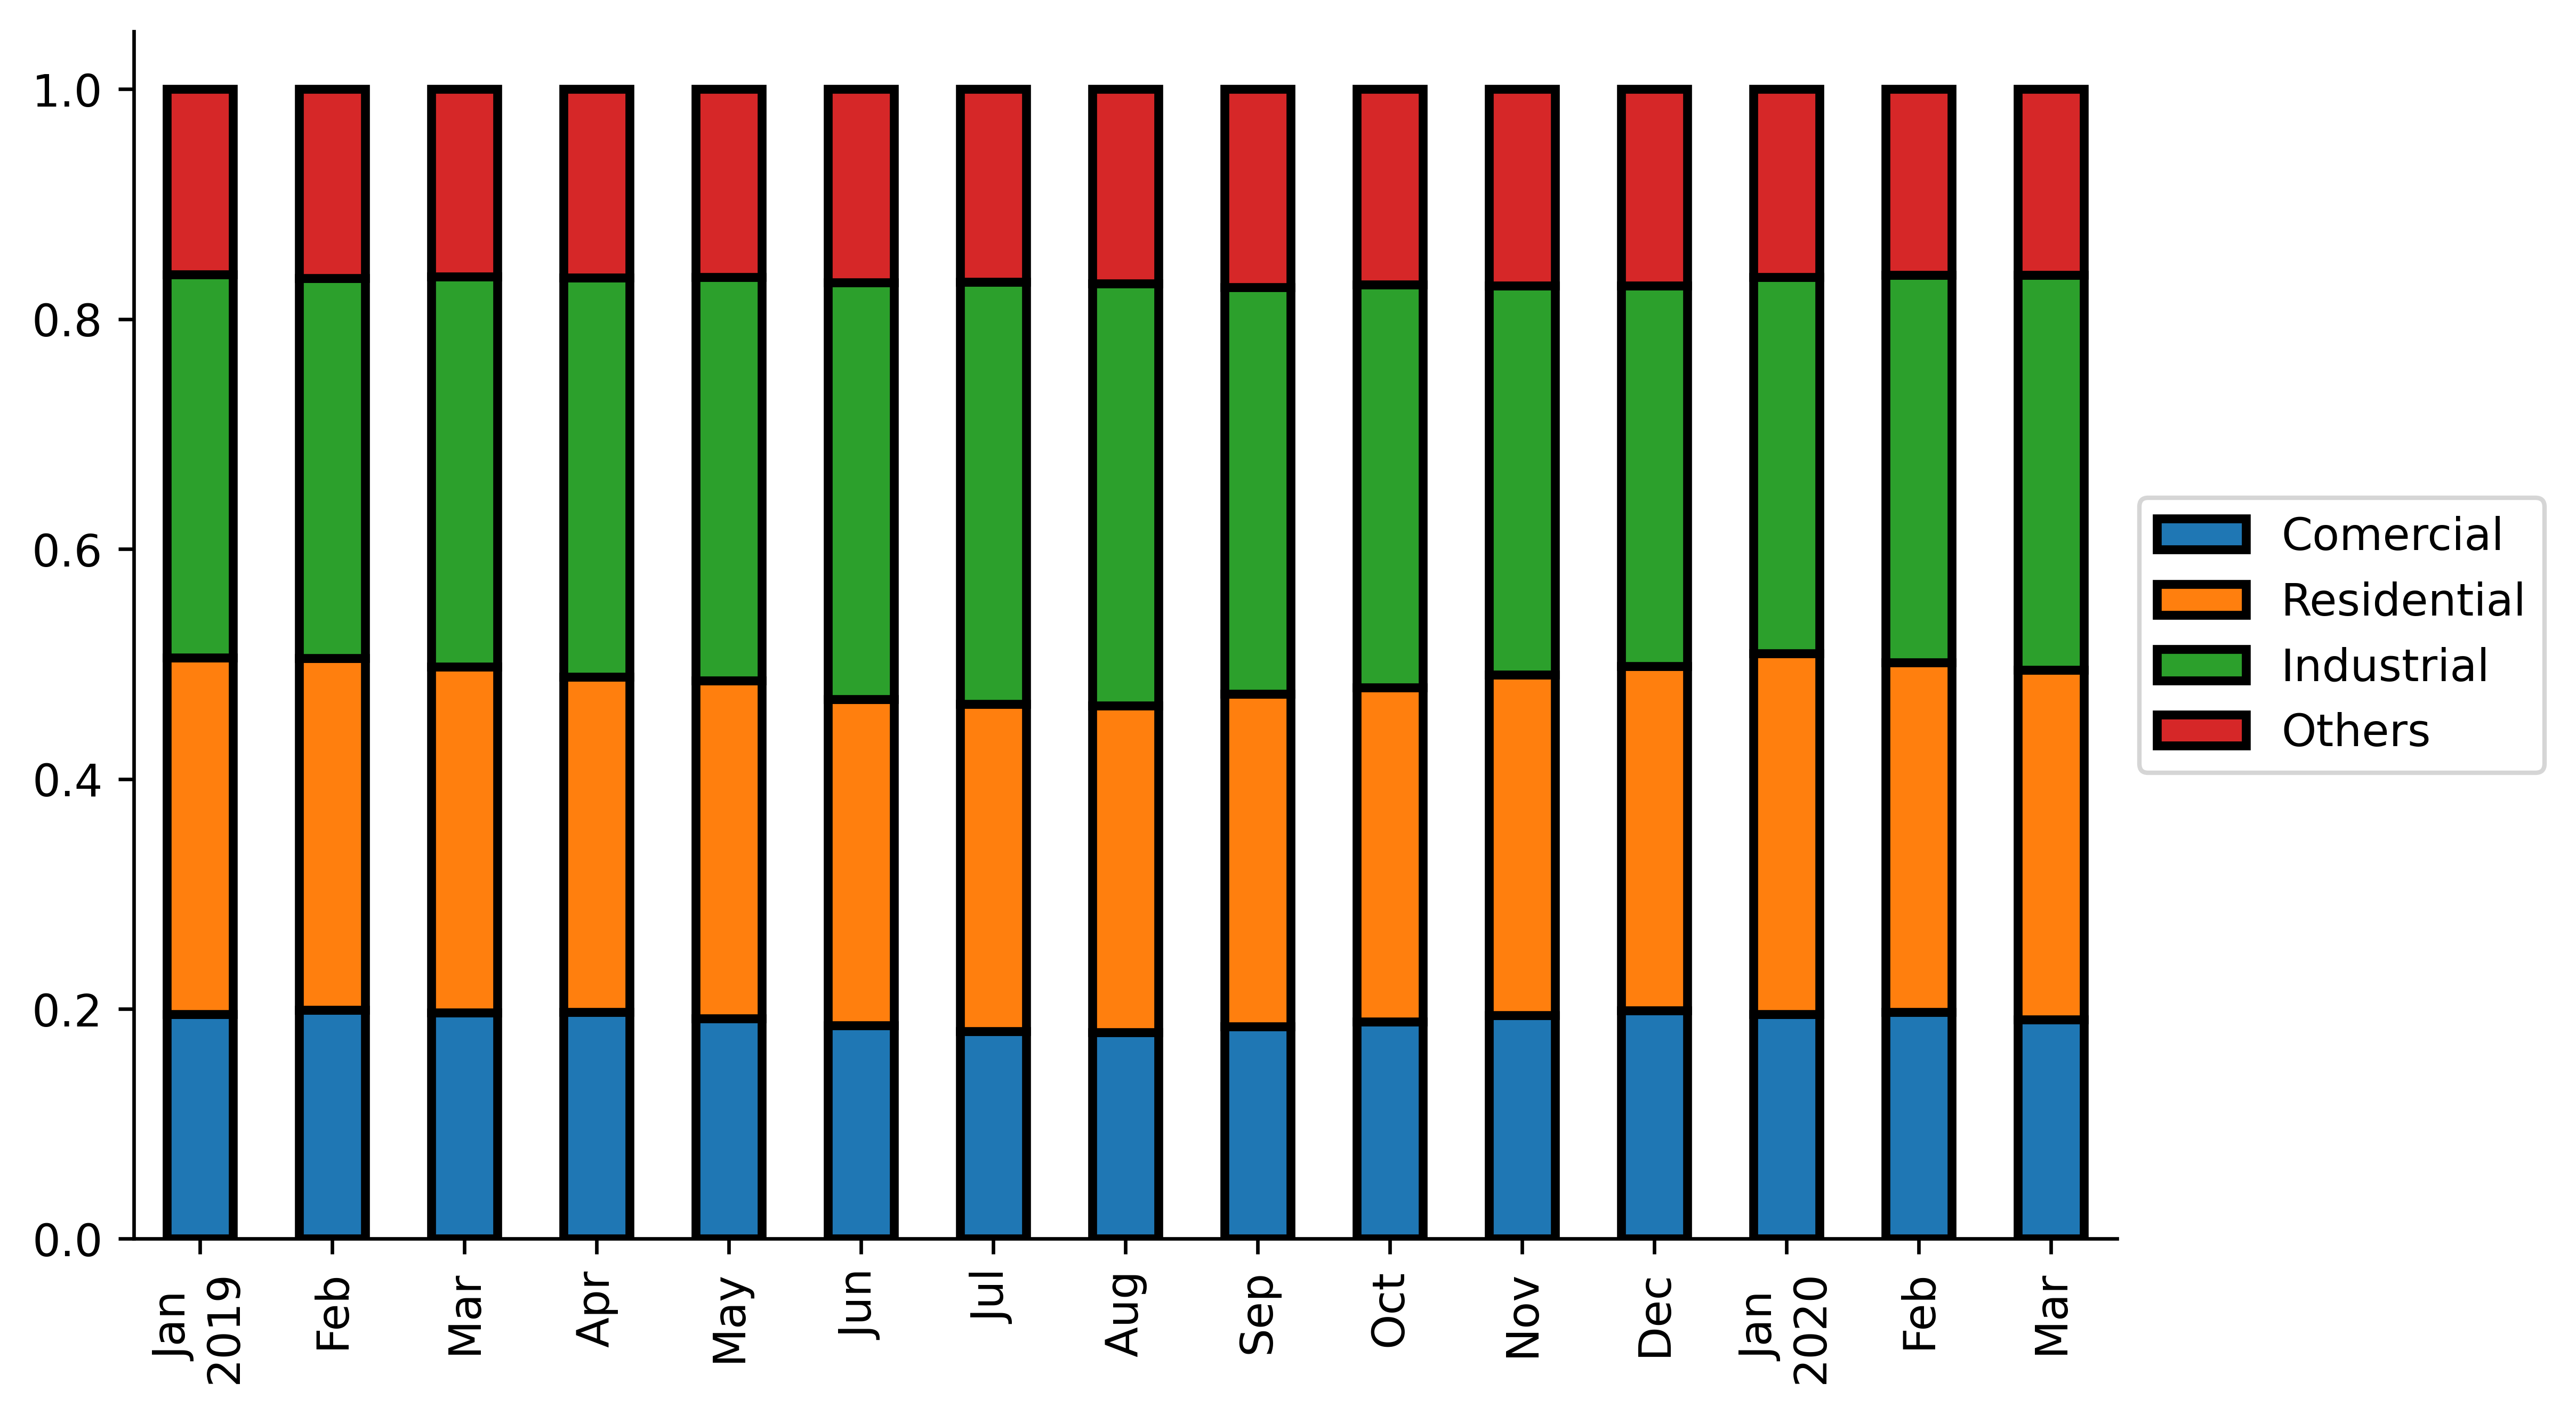
\includegraphics[width=.9\linewidth]{obipy-resources/62e383af79e91b63c7fc98dd7fb55b3c3ececcb9/b9bb93431770d5b32665b50dc4549f5f948c88a6.png}
\end{center}

\item Consumo Diário
\label{sec:org03e532b}

\begin{verbatim}
<Figure size 2400x1500 with 2 Axes>
\end{verbatim}


\begin{center}
\includegraphics[width=.9\linewidth]{obipy-resources/62e383af79e91b63c7fc98dd7fb55b3c3ececcb9/7842ed75178c7e85bc72397985d10bb7c08c16b2.png}
\end{center}

\begin{verbatim}
<Figure size 2400x1500 with 2 Axes>
\end{verbatim}


\begin{center}
\includegraphics[width=.9\linewidth]{obipy-resources/62e383af79e91b63c7fc98dd7fb55b3c3ececcb9/644bc69ef009a28fef2b58b5d83a478f7e1a78d9.png}
\end{center}

\begin{verbatim}
<Figure size 2400x1500 with 2 Axes>
\end{verbatim}


\begin{center}
\includegraphics[width=.9\linewidth]{obipy-resources/62e383af79e91b63c7fc98dd7fb55b3c3ececcb9/074f94e05c64e283dd031070baceb58c8aabbe31.png}
\end{center}

\begin{verbatim}
<Figure size 2400x1500 with 2 Axes>
\end{verbatim}


\begin{center}
\includegraphics[width=.9\linewidth]{obipy-resources/62e383af79e91b63c7fc98dd7fb55b3c3ececcb9/141e7f82711e70af2d2957c58961222b23afedb2.png}
\end{center}

\begin{verbatim}
<Figure size 2400x1500 with 2 Axes>
\end{verbatim}


\begin{center}
\includegraphics[width=.9\linewidth]{obipy-resources/62e383af79e91b63c7fc98dd7fb55b3c3ececcb9/65596f3f9ad5ba0a8bcb61d9f262ec094485ec1c.png}
\end{center}

\begin{verbatim}
<Figure size 2400x1500 with 2 Axes>
\end{verbatim}


\begin{center}
\includegraphics[width=.9\linewidth]{obipy-resources/62e383af79e91b63c7fc98dd7fb55b3c3ececcb9/2d14c6fbb2fc52f703f623c27e1b033856529304.png}
\end{center}
\end{enumerate}




\subsubsection{France: FRA}
\label{sec:orga1c2540}

<ipython-input-2-06392b792fc4>:74: UserWarning: This figure includes Axes that are not compatible with tight\_layout, so results might be incorrect.
  plt.tight\_layout()

\begin{verbatim}
<Figure size 2400x1500 with 4 Axes>
\end{verbatim}


\begin{center}
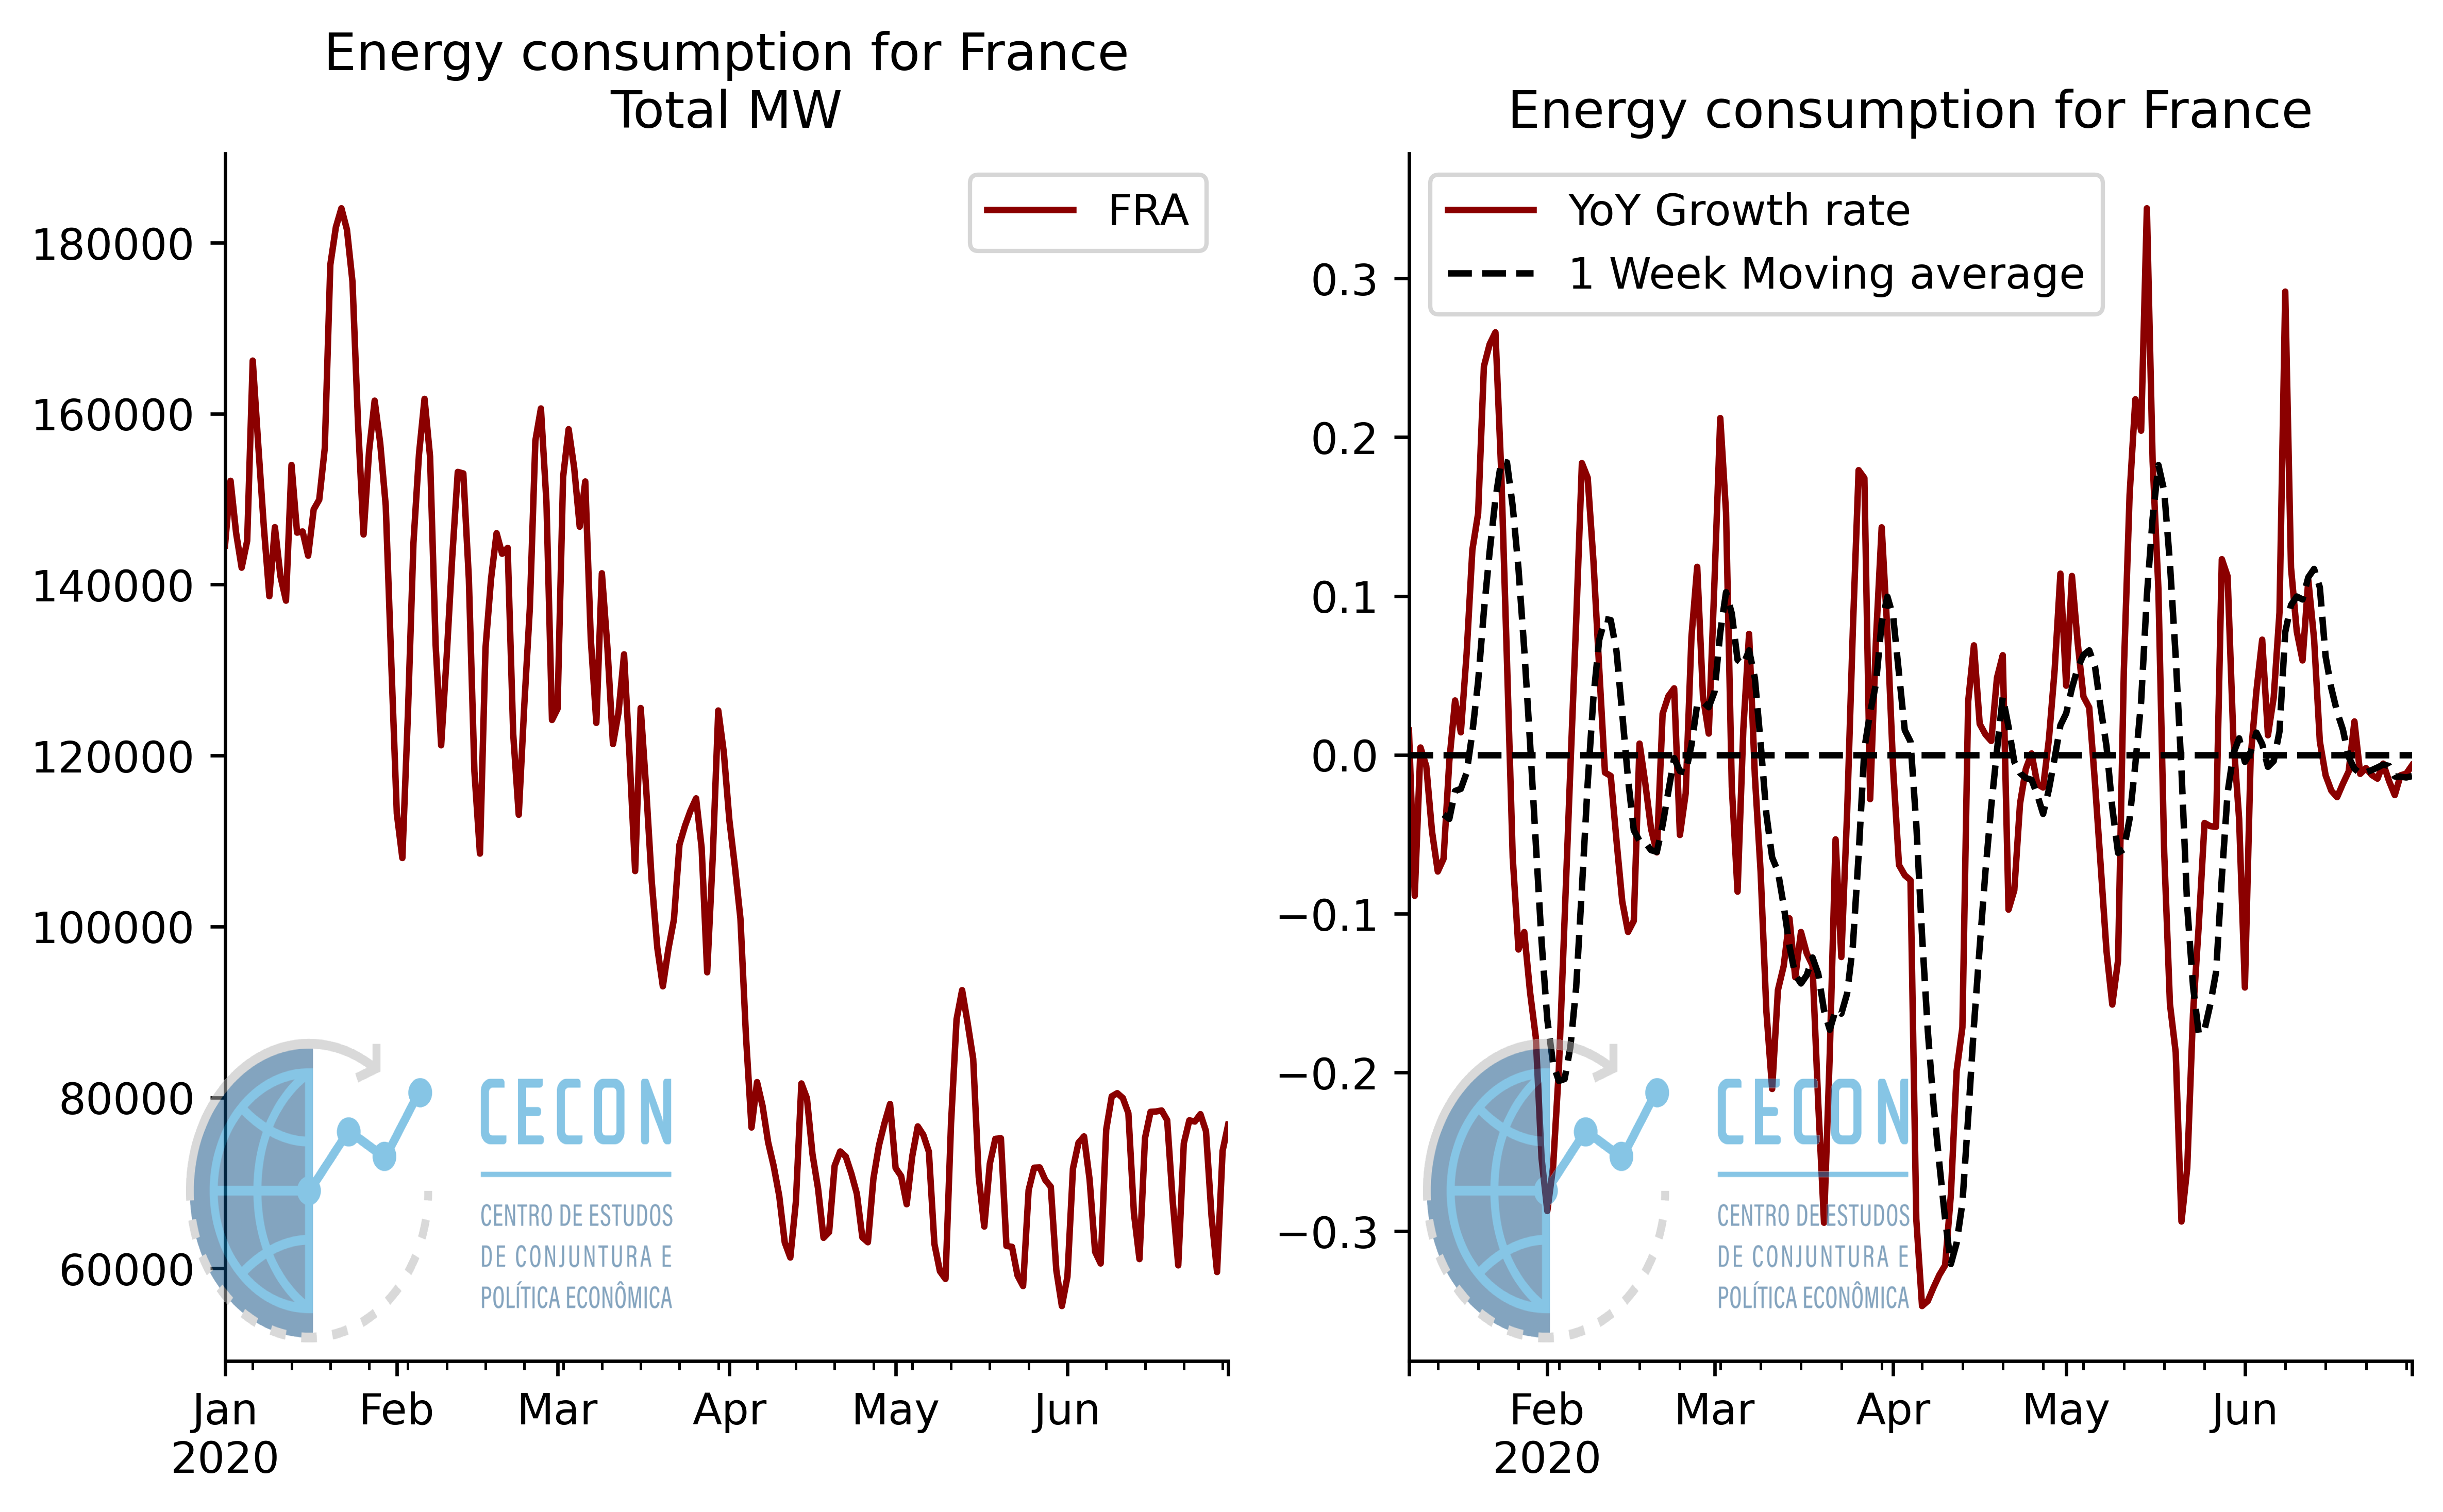
\includegraphics[width=.9\linewidth]{obipy-resources/62e383af79e91b63c7fc98dd7fb55b3c3ececcb9/325746abff053090d5f6fe9490ccdb4ba397472d.png}
\end{center}

\subsubsection{Spain: Spain}
\label{sec:orgfcc27e1}

\textbf{Corrigir}

5 - 7affede1-0db6-473c-8edf-f88f497af914 <output> <interrupt>

\subsubsection{Austria: AUS}
\label{sec:org034e0c1}

<ipython-input-2-06392b792fc4>:74: UserWarning: This figure includes Axes that are not compatible with tight\_layout, so results might be incorrect.
  plt.tight\_layout()

\begin{verbatim}
(<Figure size 2400x1500 with 4 Axes>,
 array([<matplotlib.axes._subplots.AxesSubplot object at 0x7f533d4bb130>,
        <matplotlib.axes._subplots.AxesSubplot object at 0x7f5340dc25e0>],
       dtype=object))
\end{verbatim}


\begin{verbatim}
<Figure size 2400x1500 with 4 Axes>
\end{verbatim}


\begin{center}
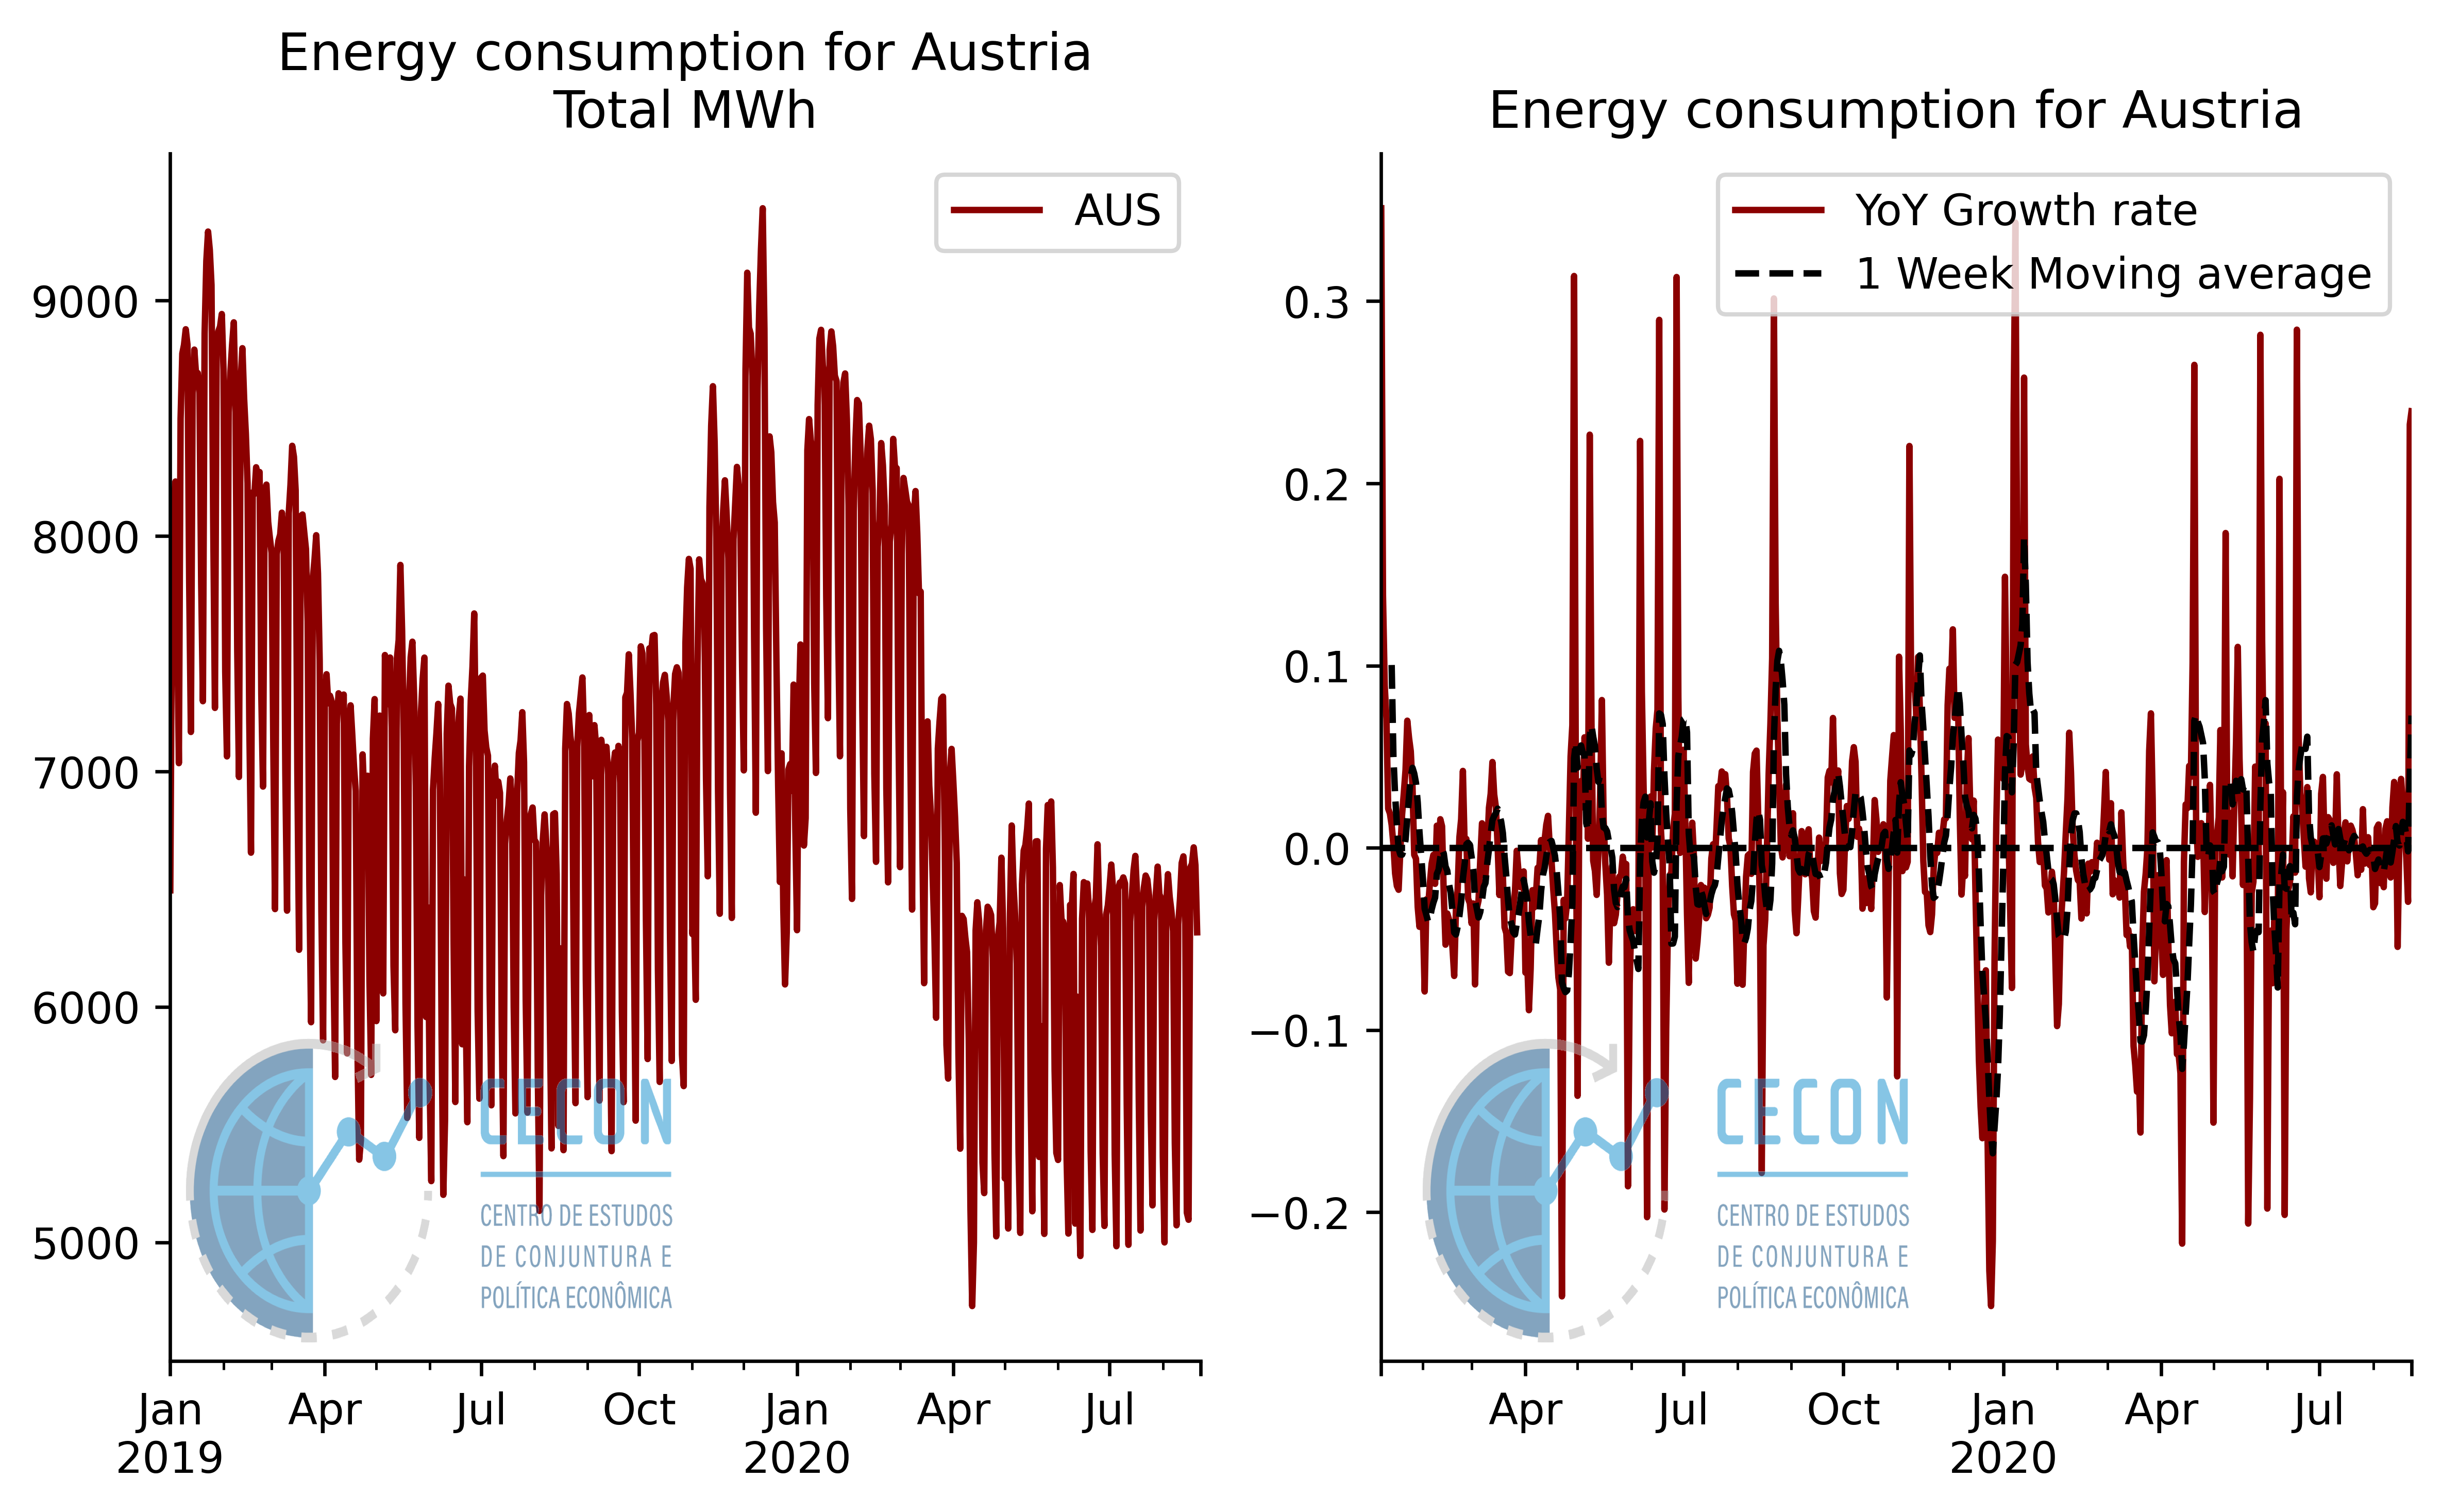
\includegraphics[width=.9\linewidth]{obipy-resources/62e383af79e91b63c7fc98dd7fb55b3c3ececcb9/9ef112a5872cc34e81a6bb8ef5d1a8c7b5fddf8e.png}
\end{center}

\subsubsection{Germany: GER}
\label{sec:org3fba5dc}

<ipython-input-2-06392b792fc4>:74: UserWarning: This figure includes Axes that are not compatible with tight\_layout, so results might be incorrect.
  plt.tight\_layout()

\begin{verbatim}
<Figure size 2400x1500 with 4 Axes>
\end{verbatim}


\begin{center}
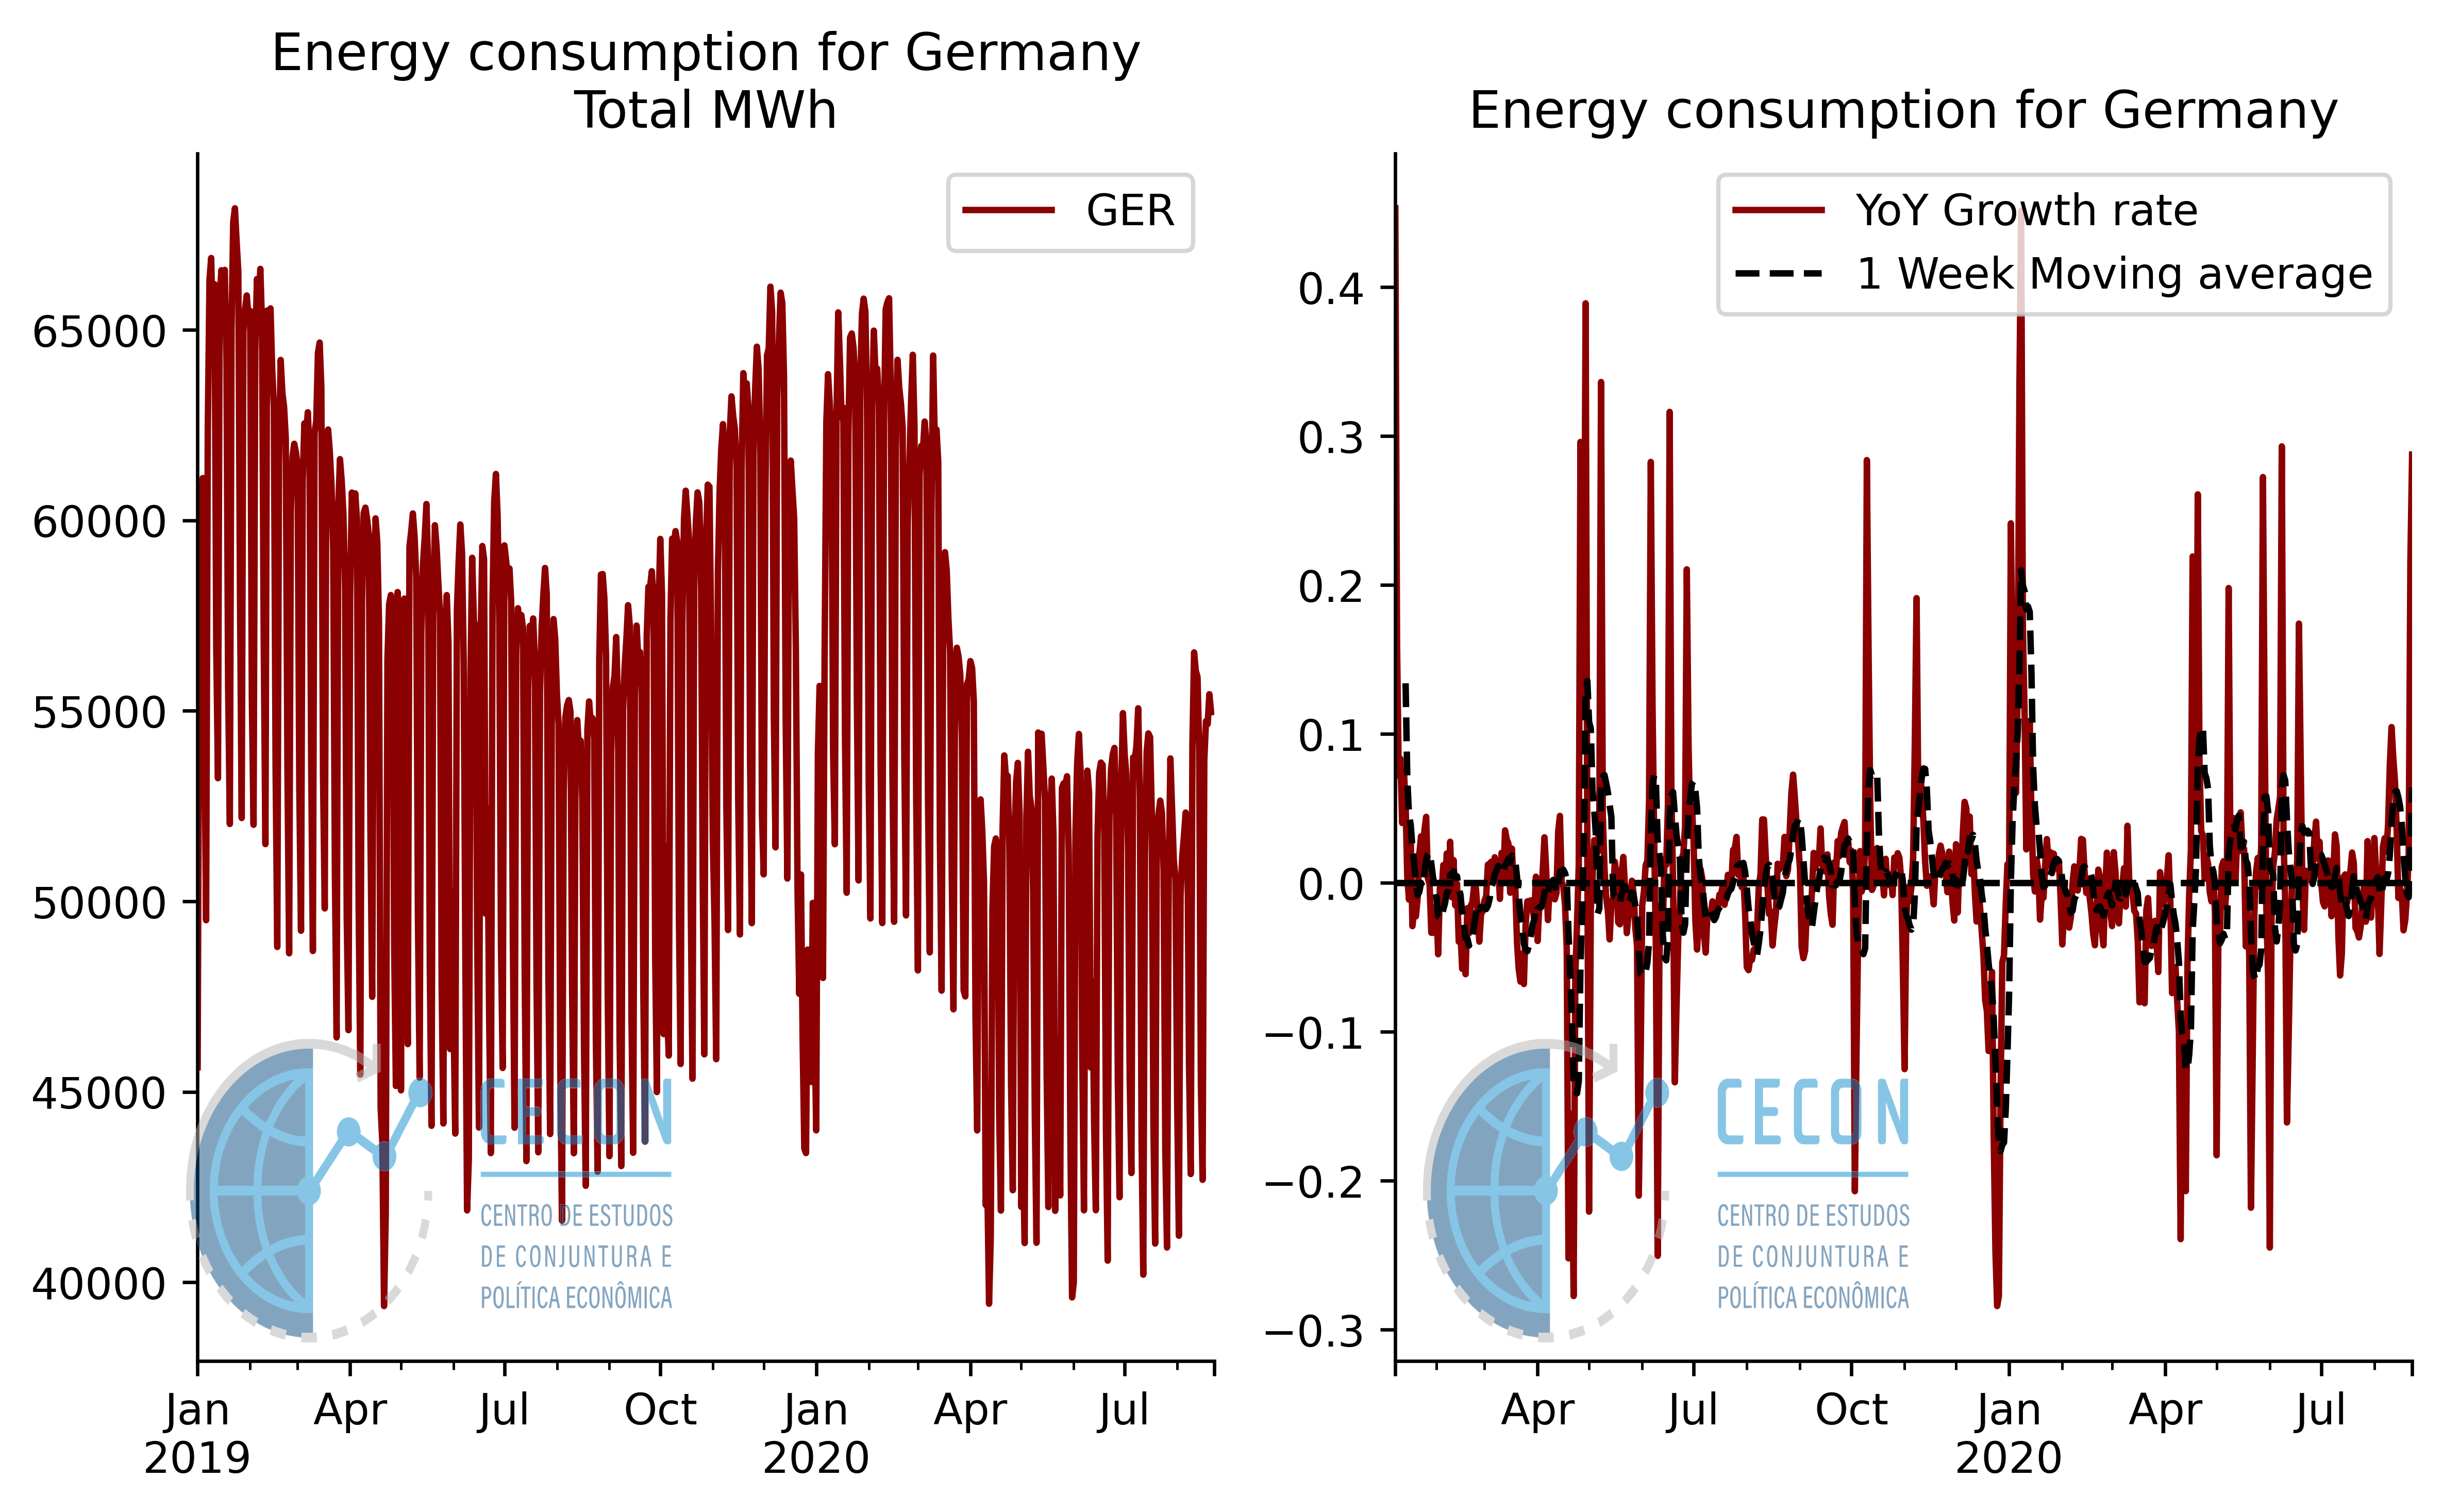
\includegraphics[width=.9\linewidth]{obipy-resources/62e383af79e91b63c7fc98dd7fb55b3c3ececcb9/94b114813ade8f5d4312e2e75f5b997a956c4a44.png}
\end{center}

\subsubsection{Luxemburg: LUX}
\label{sec:orge4f75ef}

<ipython-input-2-06392b792fc4>:74: UserWarning: This figure includes Axes that are not compatible with tight\_layout, so results might be incorrect.
  plt.tight\_layout()

\begin{verbatim}
<Figure size 2400x1500 with 4 Axes>
\end{verbatim}


\begin{center}
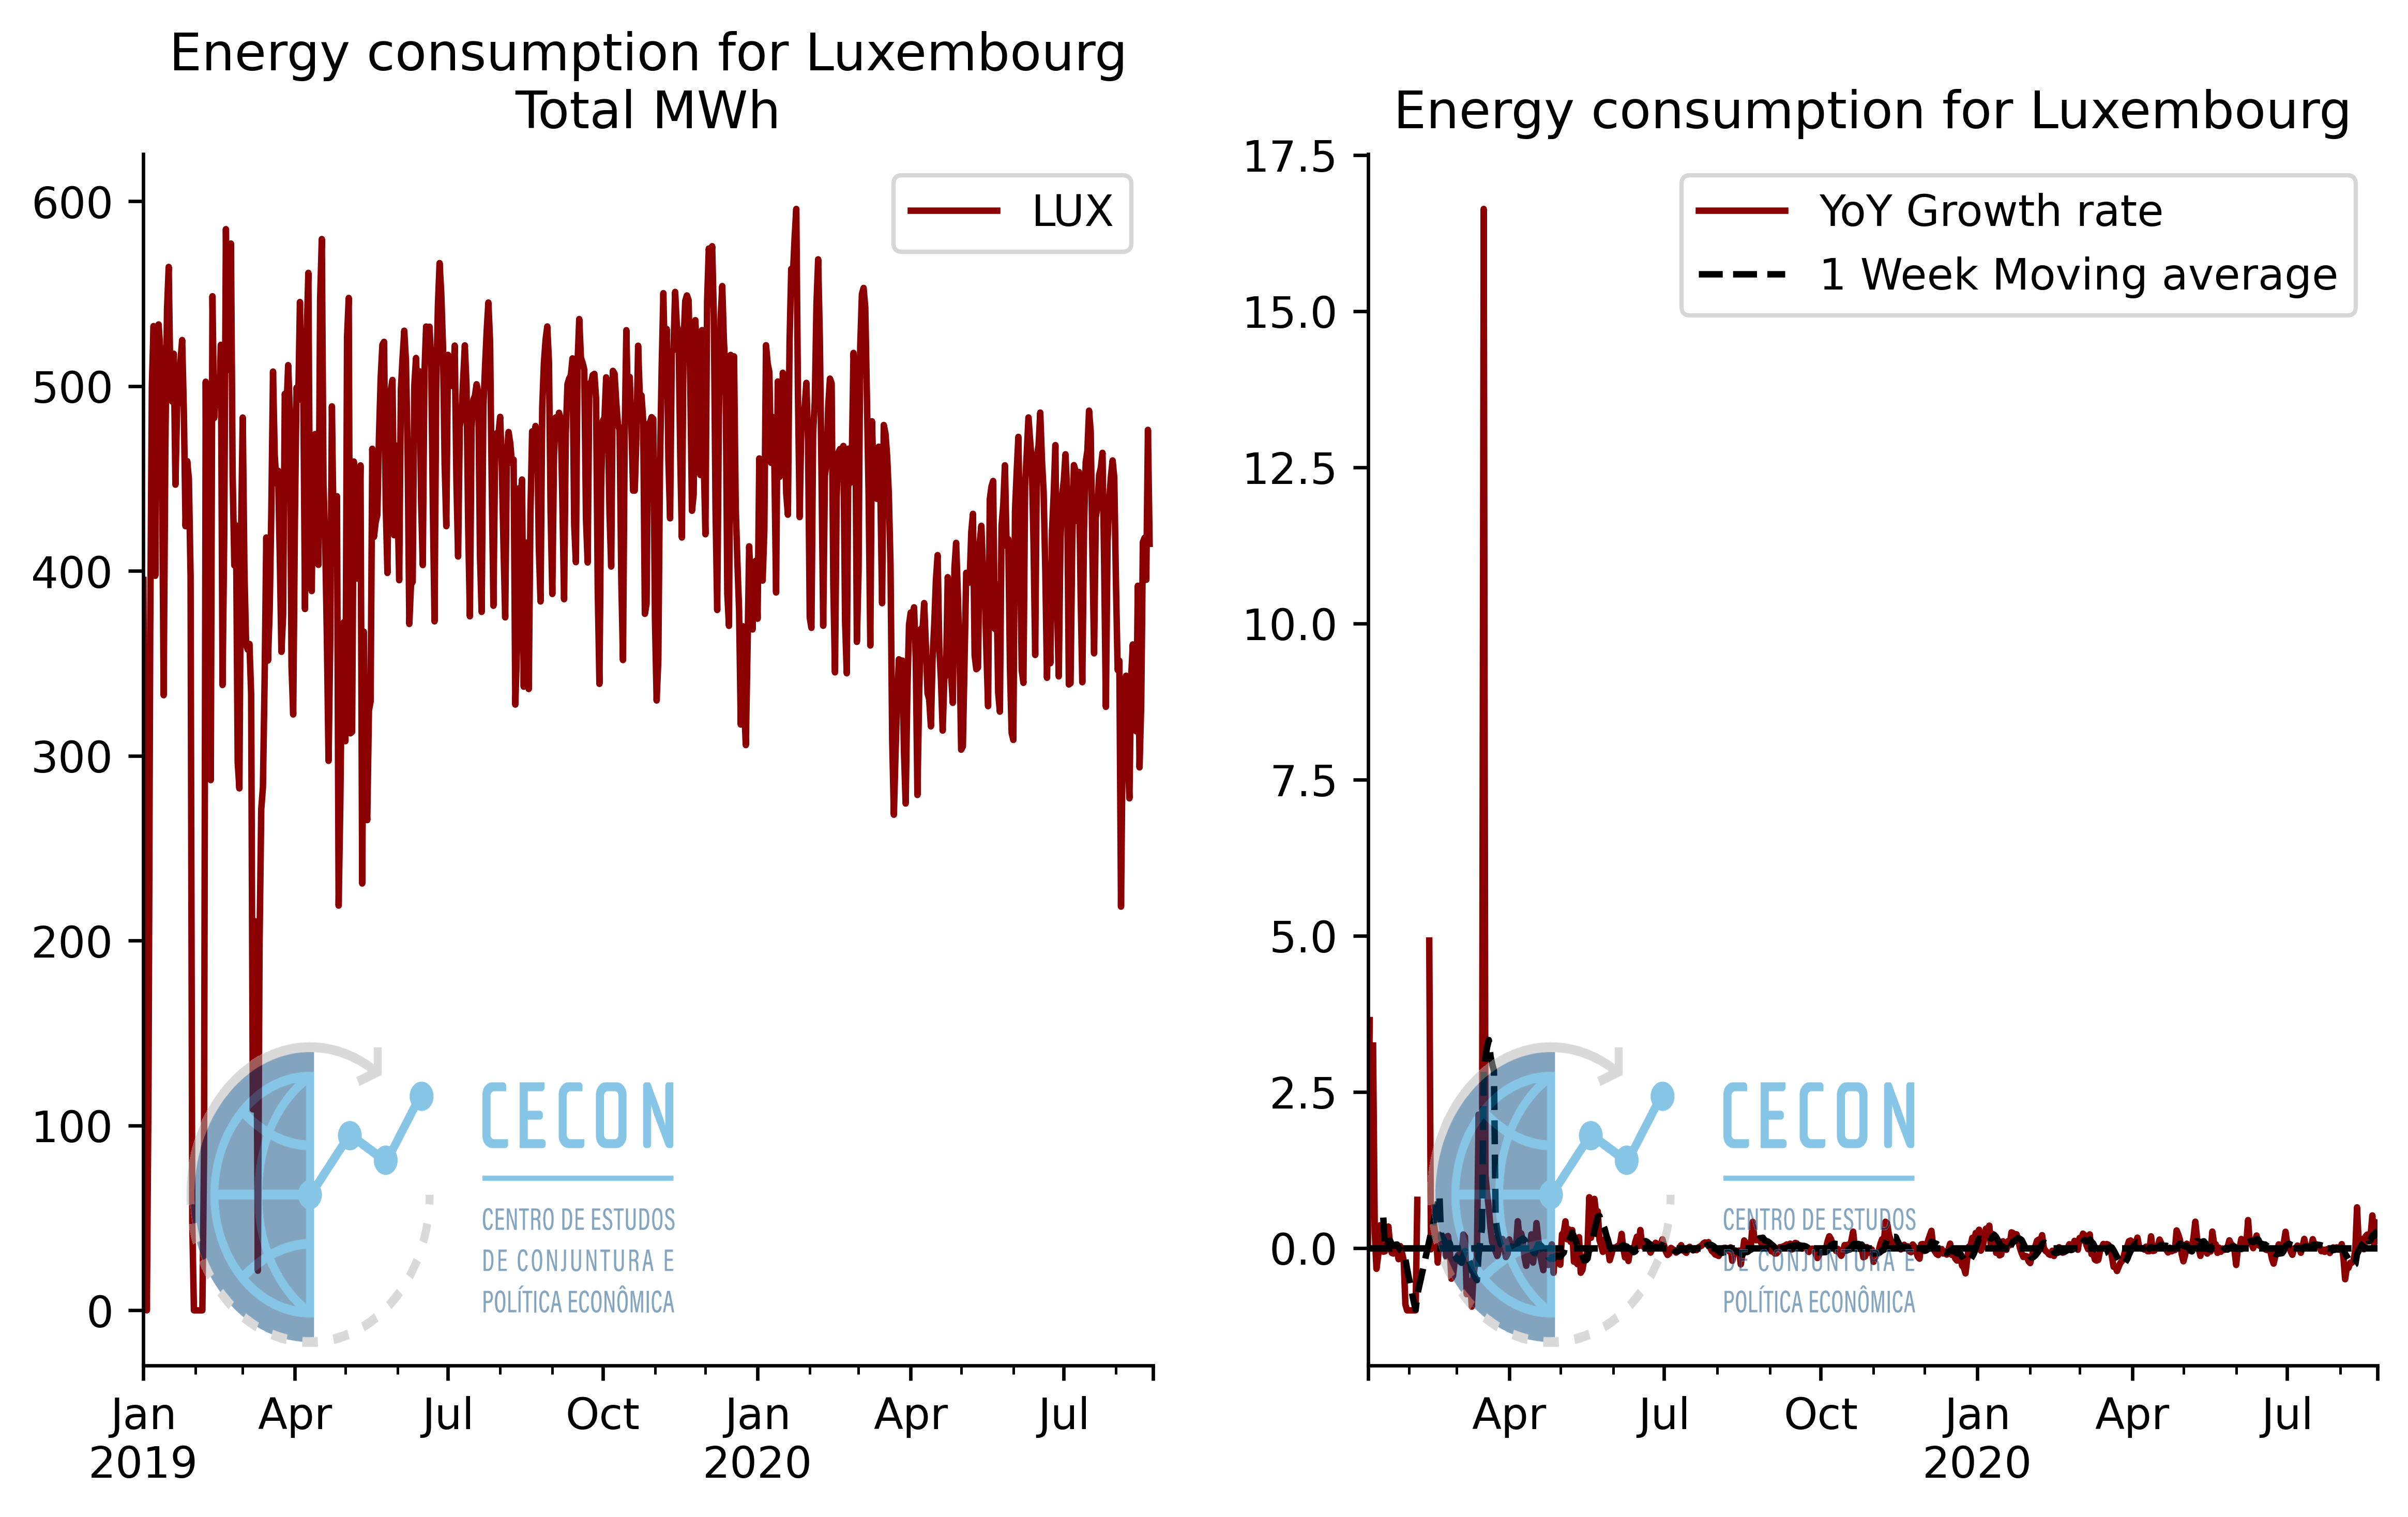
\includegraphics[width=.9\linewidth]{obipy-resources/62e383af79e91b63c7fc98dd7fb55b3c3ececcb9/9106e308f42f1f76c029539778f3952a7f562f15.png}
\end{center}


\subsection{Aruoba-Diebold-Scotti Business Conditions Index}
\label{sec:org5d58537}

\begin{verbatim}
<Figure size 2400x1500 with 2 Axes>
\end{verbatim}


\begin{center}
\includegraphics[width=.9\linewidth]{obipy-resources/62e383af79e91b63c7fc98dd7fb55b3c3ececcb9/62ce7f05bfc212f03c891e294656997d84c5d3d1.png}
\end{center}

\section{Confiança, Indicadores de antecedentes e de Risco}
\label{sec:orgd23c0ff}

\subsection{Confiança}
\label{sec:org4bd21a3}


\subsubsection{Sondagem Conjuntural Mensal}
\label{sec:orge7ce4b1}

\begin{verbatim}
<Figure size 576x360 with 2 Axes>
\end{verbatim}


\begin{center}
\includegraphics[width=.9\linewidth]{obipy-resources/62e383af79e91b63c7fc98dd7fb55b3c3ececcb9/8a25efae9231056627de37bc9a8ba5ccbde9d524.png}
\end{center}

\subsubsection{Sondagens de serviços}
\label{sec:orgd7e0ea3}

\begin{verbatim}
<Figure size 576x360 with 2 Axes>
\end{verbatim}


\begin{center}
\includegraphics[width=.9\linewidth]{obipy-resources/62e383af79e91b63c7fc98dd7fb55b3c3ececcb9/b8884fa0650b2c2def8988d527bbeadc933c5cac.png}
\end{center}


\subsubsection{Sondagem do comércio}
\label{sec:orgaeb74f8}

\begin{verbatim}
<Figure size 576x360 with 2 Axes>
\end{verbatim}


\begin{center}
\includegraphics[width=.9\linewidth]{obipy-resources/62e383af79e91b63c7fc98dd7fb55b3c3ececcb9/3ff0b698bb29513242319b177af1c0a29f2409fb.png}
\end{center}

\subsubsection{Sondagem da construção}
\label{sec:org5e24c14}

\begin{verbatim}
<Figure size 576x360 with 2 Axes>
\end{verbatim}


\begin{center}
\includegraphics[width=.9\linewidth]{obipy-resources/62e383af79e91b63c7fc98dd7fb55b3c3ececcb9/3457739c82986a176433fecd8d1a1f246d2a7529.png}
\end{center}

\subsubsection{Sondagem industrial CNI}
\label{sec:org1be52cf}


\begin{enumerate}
\item Volume de produção
\label{sec:orgee94c47}

\begin{verbatim}
<Figure size 576x360 with 2 Axes>
\end{verbatim}


\begin{center}
\includegraphics[width=.9\linewidth]{obipy-resources/62e383af79e91b63c7fc98dd7fb55b3c3ececcb9/190c8feb1adde26683c40b65c19eda8712bdf352.png}
\end{center}

\item Evolução do Emprego
\label{sec:org6f319ff}

\begin{verbatim}
<Figure size 576x360 with 2 Axes>
\end{verbatim}


\begin{center}
\includegraphics[width=.9\linewidth]{obipy-resources/62e383af79e91b63c7fc98dd7fb55b3c3ececcb9/433a12bb8c07cd8a313c63f9fd67450df4f145d1.png}
\end{center}


\item NUCI
\label{sec:org66a4487}

\noindent\rule{\textwidth}{0.5pt}
NameError                                 Traceback (most recent call last)
<ipython-input-81-f5ad43e4d316> in <module>
      9     lw = 2.5
     10 )
---> 11 ax.axvline(x = corona, color='black', ls='--', lw=1, label='Início do isolamento em SP\n(24 de março)')
     12 ax.legend(loc='center left', bbox\_to\_anchor=(1, 0.5))
     13 ax2 = plt.axes([0.135,0.135,0.2,0.2])

NameError: name 'corona' is not defined

\begin{verbatim}
<Figure size 576x360 with 1 Axes>
\end{verbatim}


\begin{center}
\includegraphics[width=.9\linewidth]{obipy-resources/62e383af79e91b63c7fc98dd7fb55b3c3ececcb9/4f9cc42543a2d57e44823ebbc3883c2e481fd6ce.png}
\end{center}

\item NUCI Efeito-Usual
\label{sec:org2a99217}

\begin{verbatim}
<Figure size 576x360 with 2 Axes>
\end{verbatim}


\begin{center}
\includegraphics[width=.9\linewidth]{obipy-resources/62e383af79e91b63c7fc98dd7fb55b3c3ececcb9/ab35061abeddc7db0e957552c2e5902ec47c321e.png}
\end{center}

\item Evolução de estoques
\label{sec:org14cc93d}

\noindent\rule{\textwidth}{0.5pt}
NameError                                 Traceback (most recent call last)
<ipython-input-83-bd6352613dfc> in <module>
      9     lw = 2.5
     10 )
---> 11 ax.axvline(x = corona, color='black', ls='--', lw=1, label='Início do isolamento em SP\n(24 de março)')
     12 ax.legend(loc='center left', bbox\_to\_anchor=(1, 0.5))
     13 ax2 = plt.axes([0.135,0.135,0.2,0.2])

NameError: name 'corona' is not defined

\begin{verbatim}
<Figure size 576x360 with 1 Axes>
\end{verbatim}


\begin{center}
\includegraphics[width=.9\linewidth]{obipy-resources/62e383af79e91b63c7fc98dd7fb55b3c3ececcb9/ee2e0ef4d86c219085ca9aa8eb1df02445fc4000.png}
\end{center}

\item Estoques efetivos
\label{sec:orgcb3ca78}

\begin{verbatim}
<Figure size 576x360 with 2 Axes>
\end{verbatim}


\begin{center}
\includegraphics[width=.9\linewidth]{obipy-resources/62e383af79e91b63c7fc98dd7fb55b3c3ececcb9/5af9aa5b5d2d37338f8964e8451506dc7e1e4c53.png}
\end{center}

\item Expectativa de Demanda
\label{sec:orgd477b6c}

\begin{verbatim}
<Figure size 576x360 with 2 Axes>
\end{verbatim}


\begin{center}
\includegraphics[width=.9\linewidth]{obipy-resources/62e383af79e91b63c7fc98dd7fb55b3c3ececcb9/26cc0738ba131ee757deed5c9a90853d5ee9f94e.png}
\end{center}

\item Expectativa de Exportação
\label{sec:org57f8263}

\begin{verbatim}
<Figure size 576x360 with 2 Axes>
\end{verbatim}


\begin{center}
\includegraphics[width=.9\linewidth]{obipy-resources/62e383af79e91b63c7fc98dd7fb55b3c3ececcb9/fb4b9ac7d589651ae78f9cb61d45452a1c20cffc.png}
\end{center}

\item Expectativa de compra de matéria-prima
\label{sec:orgb91b58f}


\begin{verbatim}
<Figure size 576x360 with 2 Axes>
\end{verbatim}


\begin{center}
\includegraphics[width=.9\linewidth]{obipy-resources/62e383af79e91b63c7fc98dd7fb55b3c3ececcb9/1613740d59e200de1ed90cd00658aa98d76fccf5.png}
\end{center}

\item Expectativa de emprego
\label{sec:orgf0945fa}

\begin{verbatim}
<Figure size 576x360 with 2 Axes>
\end{verbatim}


\begin{center}
\includegraphics[width=.9\linewidth]{obipy-resources/62e383af79e91b63c7fc98dd7fb55b3c3ececcb9/0a3e42b80d0eaee635069c6ee57ed7964c2109a5.png}
\end{center}

\item Expectativa de investimento
\label{sec:org7d5de18}

\begin{verbatim}
<Figure size 576x360 with 2 Axes>
\end{verbatim}


\begin{center}
\includegraphics[width=.9\linewidth]{obipy-resources/62e383af79e91b63c7fc98dd7fb55b3c3ececcb9/30862091e2f2a14c212ea33ba93271329494e654.png}
\end{center}

\item Lucro Operacional
\label{sec:org202765e}


\begin{verbatim}
<Figure size 576x360 with 2 Axes>
\end{verbatim}


\begin{center}
\includegraphics[width=.9\linewidth]{obipy-resources/62e383af79e91b63c7fc98dd7fb55b3c3ececcb9/e275139cf83d1eda006dc4b30dbadda64774133a.png}
\end{center}

\item Situação Financeira
\label{sec:org9acb9cb}

\begin{verbatim}
<Figure size 576x360 with 2 Axes>
\end{verbatim}


\begin{center}
\includegraphics[width=.9\linewidth]{obipy-resources/62e383af79e91b63c7fc98dd7fb55b3c3ececcb9/22bcc5c077b1cb4dcefe2a59c9d0116b7de82c73.png}
\end{center}


\item Acesso a Crédito
\label{sec:org6400384}

\begin{verbatim}
<Figure size 576x360 with 2 Axes>
\end{verbatim}


\begin{center}
\includegraphics[width=.9\linewidth]{obipy-resources/62e383af79e91b63c7fc98dd7fb55b3c3ececcb9/2ded59c6ca4da81dd78c570c38c84f405c7e65b6.png}
\end{center}
\end{enumerate}

\subsection{Indicadores de antecedente}
\label{sec:org48c1bea}

\subsubsection{Composite Leading index (\href{https://stats.oecd.org/Index.aspx?DataSetCode=MEI\_CLI}{CLI})}
\label{sec:orgf6116c8}

WARNING:root:OECD + Major Six NME not found in regex
WARNING:root:Major Five Asia not found in regex
WARNING:root:Four Big European not found in regex
WARNING:root:G7 not found in ISO2
WARNING:root:NAFTA not found in regex
WARNING:root:OECD - Total not found in regex
WARNING:root:OECD - Europe not found in regex
WARNING:root:Euro area (19 countries) not found in regex
WARNING:root:OECD total  not found in regex

\begin{verbatim}
<Figure size 576x360 with 1 Axes>
\end{verbatim}


\begin{center}
\includegraphics[width=.9\linewidth]{obipy-resources/62e383af79e91b63c7fc98dd7fb55b3c3ececcb9/4e44c8c8a59b84764b8fc9762999b8d5972932ce.png}
\end{center}


\subsubsection{Consumer Confidence index (\href{https://stats.oecd.org/Index.aspx?DataSetCode=MEI\_CCI}{CCI})}
\label{sec:org6a38dc9}

\emph{home/gpetrini}.local/lib/python3.8/site-packages/pandas/core/indexing.py:1762: PerformanceWarning: indexing past lexsort depth may impact performance.
  return self.\_getitem\_tuple(key)
WARNING:root:OECD + Major Six NME not found in regex
WARNING:root:Major Five Asia not found in regex
WARNING:root:Four Big European not found in regex
WARNING:root:G7 not found in ISO2
WARNING:root:NAFTA not found in regex
WARNING:root:OECD - Total not found in regex
WARNING:root:OECD - Europe not found in regex
WARNING:root:Euro area (19 countries) not found in regex
WARNING:root:OECD total  not found in regex

\begin{verbatim}
<Figure size 576x360 with 1 Axes>
\end{verbatim}


\begin{center}
\includegraphics[width=.9\linewidth]{obipy-resources/62e383af79e91b63c7fc98dd7fb55b3c3ececcb9/aad38e77e5fe7f43fff63b2c29856f549dc5dc3f.png}
\end{center}

\subsection{Risco}
\label{sec:orgc3c953d}

\subsubsection{EMBI+ (JP Morgan)}
\label{sec:org900a287}

\begin{verbatim}
<Figure size 576x360 with 2 Axes>
\end{verbatim}


\begin{center}
\includegraphics[width=.9\linewidth]{obipy-resources/62e383af79e91b63c7fc98dd7fb55b3c3ececcb9/8b49720c67f868a07188ddeb0242c5bb3791d599.png}
\end{center}


\subsection{Incerteza}
\label{sec:org47df873}



\subsubsection{Indicador de Incerteza (IIE-Br)}
\label{sec:org5688f53}

\begin{verbatim}
<Figure size 2400x1500 with 2 Axes>
\end{verbatim}


\begin{center}
\includegraphics[width=.9\linewidth]{obipy-resources/62e383af79e91b63c7fc98dd7fb55b3c3ececcb9/98ebb468eb299bda8f1859499b3331c18b937130.png}
\end{center}


\subsubsection{Indicador de Confiança Empresarial}
\label{sec:org3ce553f}

\begin{verbatim}
<Figure size 2400x1500 with 2 Axes>
\end{verbatim}


\begin{center}
\includegraphics[width=.9\linewidth]{obipy-resources/62e383af79e91b63c7fc98dd7fb55b3c3ececcb9/925a5b9efaef4a764499db16a51227974403bd49.png}
\end{center}

\section{Atividade}
\label{sec:org8420eae}

\subsection{Crédito}
\label{sec:org566d960}


\subsubsection{Saldo}
\label{sec:org37fd48d}

\begin{enumerate}
\item Pessoa jurídica
\label{sec:orga7d6329}

\begin{verbatim}
<Figure size 576x360 with 2 Axes>
\end{verbatim}


\begin{center}
\includegraphics[width=.9\linewidth]{obipy-resources/62e383af79e91b63c7fc98dd7fb55b3c3ececcb9/feb0adea384d3519399baabeaaea53ffd62ea8b2.png}
\end{center}


\begin{verbatim}
<Figure size 576x360 with 2 Axes>
\end{verbatim}


\begin{center}
\includegraphics[width=.9\linewidth]{obipy-resources/62e383af79e91b63c7fc98dd7fb55b3c3ececcb9/814881da38842cb94f0fd6474ddd70e90bd352da.png}
\end{center}

\item Pessoa física
\label{sec:orgacb10d0}

\begin{verbatim}
<Figure size 576x360 with 2 Axes>
\end{verbatim}


\begin{center}
\includegraphics[width=.9\linewidth]{obipy-resources/62e383af79e91b63c7fc98dd7fb55b3c3ececcb9/631784503e9693a2f771311b1a337a6f61bd3bcb.png}
\end{center}

\begin{verbatim}
<Figure size 576x360 with 2 Axes>
\end{verbatim}


\begin{center}
\includegraphics[width=.9\linewidth]{obipy-resources/62e383af79e91b63c7fc98dd7fb55b3c3ececcb9/840ea262d5c525c19284dff3d45594fc372c02d1.png}
\end{center}

\item Crédito ampliado
\label{sec:orgc04387f}

\begin{verbatim}
<Figure size 576x360 with 2 Axes>
\end{verbatim}


\begin{center}
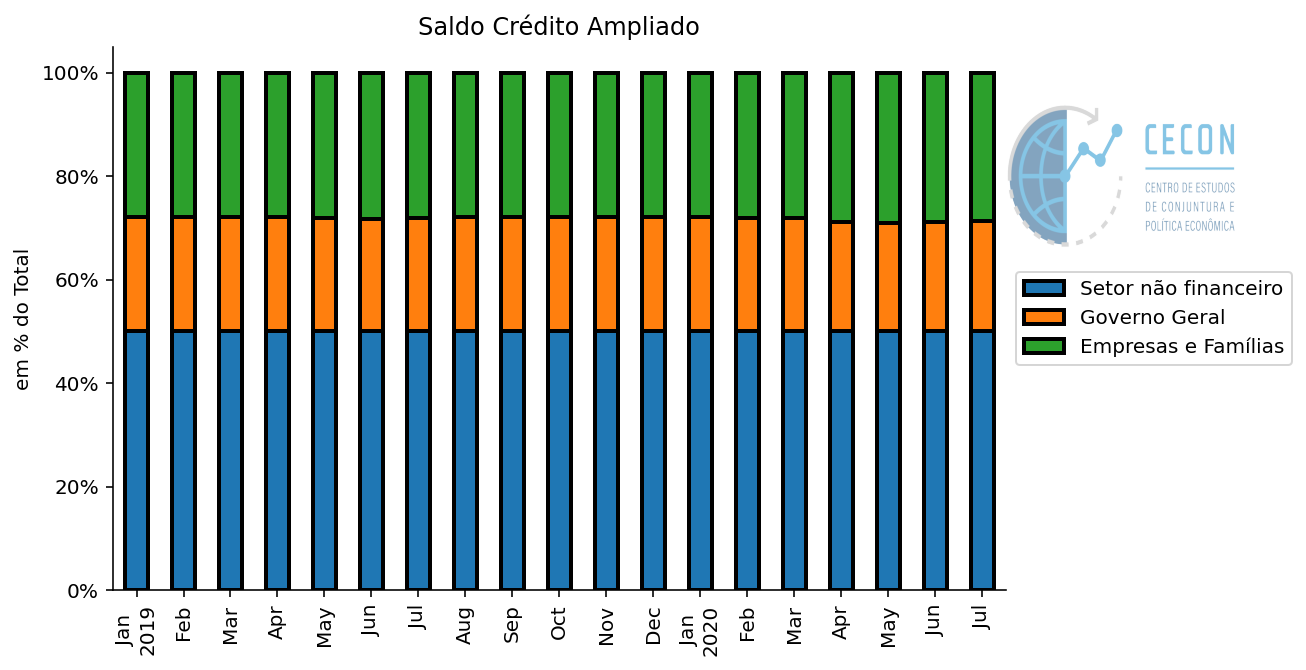
\includegraphics[width=.9\linewidth]{obipy-resources/62e383af79e91b63c7fc98dd7fb55b3c3ececcb9/fc25f4901d8007b52b37c8cc10e4620bc37873f2.png}
\end{center}

\begin{verbatim}
<Figure size 576x360 with 2 Axes>
\end{verbatim}


\begin{center}
\includegraphics[width=.9\linewidth]{obipy-resources/62e383af79e91b63c7fc98dd7fb55b3c3ececcb9/d787c0b50fa6cabeff88eb82b75849ce6f26ce84.png}
\end{center}


\begin{verbatim}
<Figure size 576x360 with 2 Axes>
\end{verbatim}


\begin{center}
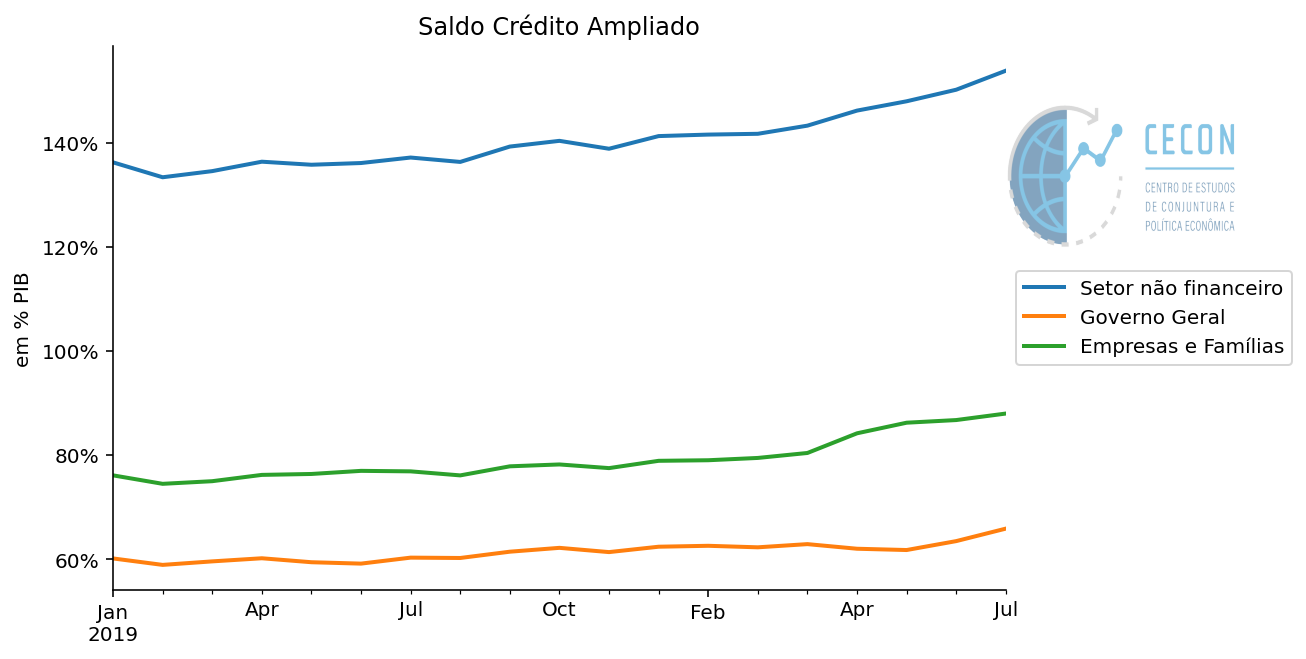
\includegraphics[width=.9\linewidth]{obipy-resources/62e383af79e91b63c7fc98dd7fb55b3c3ececcb9/71e2f6f170d1eae4c7e08b6bb69381e2fc6bfa43.png}
\end{center}

\item Crédito direcionado
\label{sec:org598c4e8}


\begin{verbatim}
<Figure size 576x360 with 2 Axes>
\end{verbatim}


\begin{center}
\includegraphics[width=.9\linewidth]{obipy-resources/62e383af79e91b63c7fc98dd7fb55b3c3ececcb9/ce90c1989329de9bd35e54499a49e998a229e167.png}
\end{center}

\begin{verbatim}
<Figure size 576x360 with 2 Axes>
\end{verbatim}


\begin{center}
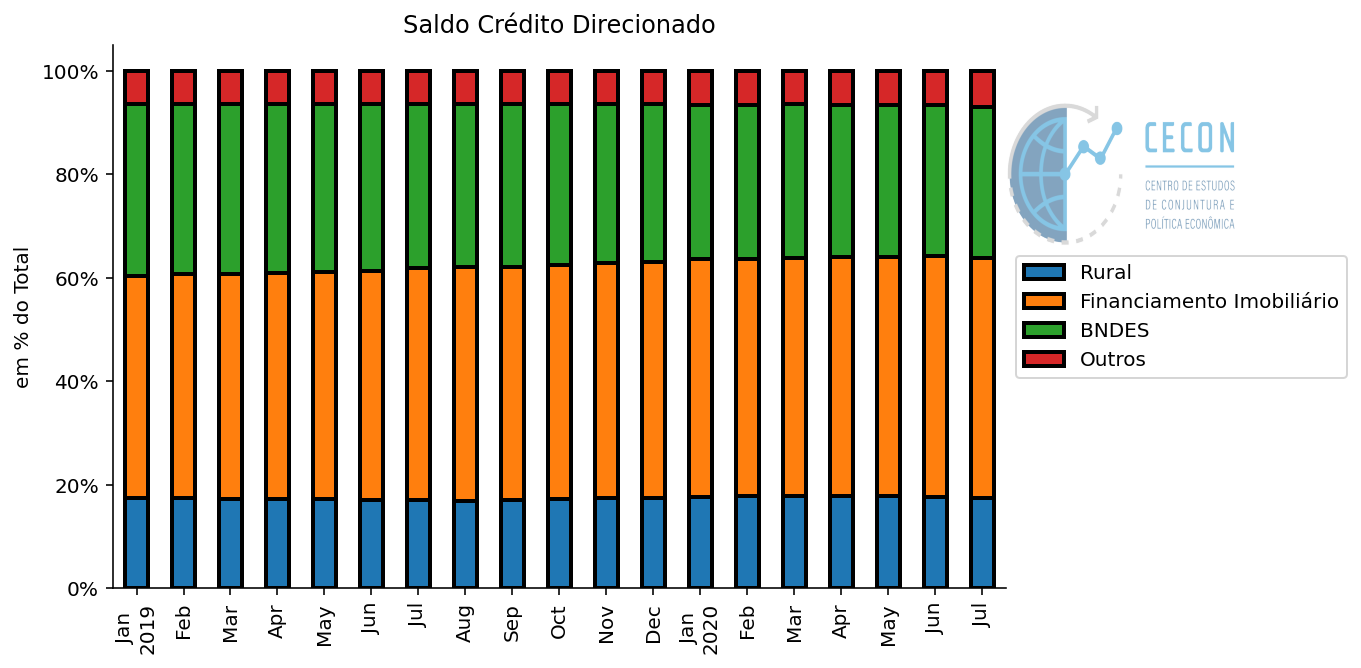
\includegraphics[width=.9\linewidth]{obipy-resources/62e383af79e91b63c7fc98dd7fb55b3c3ececcb9/9a2b55ba48387fe773ae71f452b084dae90c5a91.png}
\end{center}

\begin{verbatim}
<Figure size 576x360 with 2 Axes>
\end{verbatim}


\begin{center}
\includegraphics[width=.9\linewidth]{obipy-resources/62e383af79e91b63c7fc98dd7fb55b3c3ececcb9/120b087dfcc6ee8bca3227ec45868b7327bde212.png}
\end{center}
\end{enumerate}



\subsection{IBCBr}
\label{sec:org095ee82}

\begin{verbatim}
<Figure size 576x360 with 2 Axes>
\end{verbatim}


\begin{center}
\includegraphics[width=.9\linewidth]{obipy-resources/62e383af79e91b63c7fc98dd7fb55b3c3ececcb9/51df5d2fc00ebe923cd476edd2384c8734922982.png}
\end{center}

\subsection{PIB (Contas Nacionais)}
\label{sec:orgf8c8987}

Archive:  Tab\_Compl\_CNT.zip
  inflating: Tab\_Compl\_CNT.xls       

\subsubsection{Trimestre Contra trimestre imediatamente anterior}
\label{sec:org0ac5918}

2019Q3    0.000588
2019Q4    0.005339
2020Q1   -0.024549
2020Q2   -0.096930
Freq: Q-DEC, Name: PIB, dtype: float64

\begin{verbatim}
<Figure size 648x288 with 2 Axes>
\end{verbatim}


\begin{center}
\includegraphics[width=.9\linewidth]{obipy-resources/62e383af79e91b63c7fc98dd7fb55b3c3ececcb9/9c59f5df2a1d798fc2f3361d06d39e748802980c.png}
\end{center}

\begin{enumerate}
\item Agropecuária
\label{sec:org70ee122}

\begin{verbatim}
<Figure size 648x288 with 2 Axes>
\end{verbatim}


\begin{center}
\includegraphics[width=.9\linewidth]{obipy-resources/62e383af79e91b63c7fc98dd7fb55b3c3ececcb9/8c82528a54963f72680dc80334272720121e728d.png}
\end{center}

\item Indústria
\label{sec:org29da86c}

        Industria Extrativa  Industria de Transformacao  Eletricidade e agua  $\backslash$
2019Q3             0.126922                   -0.009143            -0.012028   
2019Q4             0.007993                    0.001056            -0.001173   
2020Q1            -0.047379                   -0.019497            -0.003147   
2020Q2            -0.011218                   -0.175394            -0.043949   

        Construcao  Total Industria  
2019Q3    0.007231         0.005460  
2019Q4   -0.030270         0.000602  
2020Q1   -0.033302        -0.008139  
2020Q2   -0.056655        -0.122893  

\begin{verbatim}
<Figure size 648x288 with 2 Axes>
\end{verbatim}


\begin{center}
\includegraphics[width=.9\linewidth]{obipy-resources/62e383af79e91b63c7fc98dd7fb55b3c3ececcb9/176ed5c24348d0be70e4afbae6f3ebcc4591a5c8.png}
\end{center}


\item Serviços
\label{sec:org478080b}

        Comercio  Transporte, armazenagem e correio  Informacao e comunicacao  $\backslash$
1996Q1       NaN                                NaN                       NaN   
1996Q2  0.013930                          -0.022250                  0.014198   
1996Q3  0.027921                           0.032652                  0.041464   
1996Q4  0.013399                          -0.037413                 -0.024424   
1997Q1  0.000426                           0.046895                  0.015430   
\ldots{}          \ldots{}                                \ldots{}                       \ldots{}   
2019Q2  0.006191                          -0.001205                  0.014362   
2019Q3  0.004430                          -0.001166                  0.008591   
2019Q4 -0.002416                           0.012850                  0.010421   
2020Q1 -0.014039                          -0.024127                 -0.019601   
2020Q2 -0.130136                          -0.193399                 -0.029687   

        Atividades Financeiras  Atividades Imobiliarias  Outras atividades  $\backslash$
1996Q1                     NaN                      NaN                NaN   
1996Q2                0.001766                 0.006362           0.003576   
1996Q3               -0.000033                 0.009057           0.003184   
1996Q4               -0.087247                -0.024478          -0.005366   
1997Q1                0.110797                 0.022929           0.019185   
\ldots{}                        \ldots{}                      \ldots{}                \ldots{}   
2019Q2               -0.007478                 0.007306           0.000918   
2019Q3                0.016924                 0.003003          -0.000463   
2019Q4                0.008832                 0.002152           0.008042   
2020Q1                0.002412                 0.003421          -0.053256   
2020Q2                0.008441                 0.004705          -0.198343   

        ADM, defesa, etc  Total Servicos  
1996Q1               NaN             NaN  
1996Q2          0.019224        0.012489  
1996Q3          0.005550        0.014601  
1996Q4         -0.005808       -0.020523  
1997Q1         -0.000785        0.024352  
\ldots{}                  \ldots{}             \ldots{}  
2019Q2         -0.005078       -0.000415  
2019Q3         -0.006734        0.001378  
2019Q4          0.010494        0.005582  
2020Q1         -0.014418       -0.022358  
2020Q2         -0.076251       -0.097166  

[98 rows x 8 columns]

\begin{verbatim}
<Figure size 648x288 with 2 Axes>
\end{verbatim}


\begin{center}
\includegraphics[width=.9\linewidth]{obipy-resources/62e383af79e91b63c7fc98dd7fb55b3c3ececcb9/b36716a8f621c4be345ff6778cf910c669398c18.png}
\end{center}

\item Demanda
\label{sec:orgf5a1fa1}

        Consumo das Familias  Consumo do Governo      FBCF  Exportacao  $\backslash$
2019Q3              0.005088           -0.003986  0.015347   -0.022088   
2019Q4              0.003992            0.004443 -0.034854    0.023254   
2020Q1             -0.019217            0.002193  0.022937   -0.013177   
2020Q2             -0.125381           -0.088450 -0.154231    0.018445   

        Importacao       PIB  
2019Q3    0.001535  0.000588  
2019Q4   -0.025791  0.005339  
2020Q1    0.008115 -0.024549  
2020Q2   -0.132437 -0.096930  

\begin{verbatim}
<Figure size 648x288 with 2 Axes>
\end{verbatim}


\begin{center}
\includegraphics[width=.9\linewidth]{obipy-resources/62e383af79e91b63c7fc98dd7fb55b3c3ececcb9/7c327ff8eb33f8d12b7d6afbac964411bee5ec80.png}
\end{center}

\item Oferta
\label{sec:org476fd41}


        Agropecuaria  Total Industria  Total Servicos       PIB
2019Q3      0.010857         0.005460        0.001378  0.000588
2019Q4     -0.006840         0.000602        0.005582  0.005339
2020Q1      0.005004        -0.008139       -0.022358 -0.024549
2020Q2      0.004292        -0.122893       -0.097166 -0.096930

\begin{verbatim}
<Figure size 648x288 with 2 Axes>
\end{verbatim}


\begin{center}
\includegraphics[width=.9\linewidth]{obipy-resources/62e383af79e91b63c7fc98dd7fb55b3c3ececcb9/3ca4b1a3528958dfe9791cb732725b96a282c3b3.png}
\end{center}
\end{enumerate}


\subsubsection{Contribuição para variação}
\label{sec:orgdec5745}

\begin{enumerate}
\item Demanda
\label{sec:org5f4ab67}

        Consumo das Familias  Consumo do Governo      FBCF  Exportacao  $\backslash$
2018Q3              0.003670            0.000547  0.008612    0.008489   
2018Q4              0.001643           -0.002391 -0.002606    0.002801   
2019Q1              0.005201            0.001083 -0.001710   -0.005277   
2019Q2              0.002270           -0.000528  0.004948   -0.003653   
2019Q3              0.003469           -0.000725  0.002711   -0.003011   
2019Q4              0.002734            0.000805 -0.006249    0.003098   
2020Q1             -0.013143            0.000397  0.003948   -0.001787   
2020Q2             -0.086221           -0.016445 -0.027837    0.002530   

        Importacao  
2018Q3   -0.009075  
2018Q4    0.005034  
2019Q1    0.003006  
2019Q2   -0.006682  
2019Q3   -0.000221  
2019Q4    0.003713  
2020Q1   -0.001132  
2020Q2    0.019092  

\begin{verbatim}
<Figure size 432x288 with 1 Axes>
\end{verbatim}


\begin{center}
\includegraphics[width=.9\linewidth]{obipy-resources/62e383af79e91b63c7fc98dd7fb55b3c3ececcb9/e2105790570f9e49e7872b20e975495b01aa9d17.png}
\end{center}

\item Oferta
\label{sec:org215666d}

\emph{home/gpetrini}.local/lib/python3.8/site-packages/pandas/plotting/\_matplotlib/core.py:218: UserWarning: 'color' and 'colormap' cannot be used simultaneously. Using 'color'
  warnings.warn(
\emph{home/gpetrini}.local/lib/python3.8/site-packages/pandas/plotting/\_matplotlib/style.py:27: UserWarning: 'color' and 'colormap' cannot be used simultaneously. Using 'color'
  warnings.warn(
        Agropecuaria  Total Industria  Total Servicos
2018Q3      0.000785         0.000917        0.003821
2018Q4      0.000366        -0.001947       -0.001539
2019Q1     -0.000803         0.000185        0.006582
2019Q2      0.000890         0.001510       -0.000295
2019Q3      0.000863         0.001174        0.000979
2019Q4     -0.000548         0.000130        0.003963
2020Q1      0.000396        -0.001746       -0.015865
2020Q2      0.000349        -0.026782       -0.069045

\begin{verbatim}
<Figure size 648x288 with 2 Axes>
\end{verbatim}


\begin{center}
\includegraphics[width=.9\linewidth]{obipy-resources/62e383af79e91b63c7fc98dd7fb55b3c3ececcb9/e51f3a05cd7cc553d133062ba14404ab5b055f1a.png}
\end{center}
\end{enumerate}

\subsubsection{Carregamento estatístico}
\label{sec:org7615b3c}


\section{Setor Externo}
\label{sec:org52219d2}


\subsection{Balanço de Pagamentos}
\label{sec:org06a4c16}



\subsubsection{Balança comercial}
\label{sec:org7a8c758}

\begin{verbatim}
<Figure size 576x360 with 2 Axes>
\end{verbatim}


\begin{center}
\includegraphics[width=.9\linewidth]{obipy-resources/62e383af79e91b63c7fc98dd7fb55b3c3ececcb9/1e0d8385dd451046cdb0d2ba3d5177a8c0b66b09.png}
\end{center}


\begin{verbatim}
<Figure size 576x360 with 2 Axes>
\end{verbatim}


\begin{center}
\includegraphics[width=.9\linewidth]{obipy-resources/62e383af79e91b63c7fc98dd7fb55b3c3ececcb9/5c8166f4bad84dd16ebefa571131cb142728daa5.png}
\end{center}


\begin{verbatim}
<Figure size 576x360 with 2 Axes>
\end{verbatim}


\begin{center}
\includegraphics[width=.9\linewidth]{obipy-resources/62e383af79e91b63c7fc98dd7fb55b3c3ececcb9/0c79e964de2ddd1cb6e026cbcf8475b6f5849d98.png}
\end{center}


\subsubsection{Conta corrente (\%PIB)}
\label{sec:orga05351c}

\begin{verbatim}
<Figure size 576x360 with 2 Axes>
\end{verbatim}


\begin{center}
\includegraphics[width=.9\linewidth]{obipy-resources/62e383af79e91b63c7fc98dd7fb55b3c3ececcb9/1c5d34e0d8ec55b286fb4de024d0b7b11b8bcf58.png}
\end{center}

\subsubsection{Balança Comercial por país (mensal)}
\label{sec:org29762e1}

\begin{verbatim}
<Figure size 576x360 with 2 Axes>
\end{verbatim}


\begin{center}
\includegraphics[width=.9\linewidth]{obipy-resources/62e383af79e91b63c7fc98dd7fb55b3c3ececcb9/c3ff075133f390045c0fb620ae17d0d8ae93f0b8.png}
\end{center}


\begin{verbatim}
<Figure size 576x360 with 2 Axes>
\end{verbatim}


\begin{center}
\includegraphics[width=.9\linewidth]{obipy-resources/62e383af79e91b63c7fc98dd7fb55b3c3ececcb9/94e3a318f5fa3b548791774e379fcc93c0ac6151.png}
\end{center}

\begin{enumerate}
\item Importações
\label{sec:orgfe58c11}

\begin{verbatim}
<Figure size 576x360 with 2 Axes>
\end{verbatim}


\begin{center}
\includegraphics[width=.9\linewidth]{obipy-resources/62e383af79e91b63c7fc98dd7fb55b3c3ececcb9/418cb4f4d4375891918713f399f1fd90e9c5c223.png}
\end{center}


\begin{verbatim}
<Figure size 576x360 with 2 Axes>
\end{verbatim}


\begin{center}
\includegraphics[width=.9\linewidth]{obipy-resources/62e383af79e91b63c7fc98dd7fb55b3c3ececcb9/5deabc9a2c1ef0035dab475172a88f0cbcbb7efa.png}
\end{center}
\end{enumerate}


\subsubsection{Saldo Comercial}
\label{sec:org1829cc8}

\begin{verbatim}
<Figure size 576x360 with 2 Axes>
\end{verbatim}


\begin{center}
\includegraphics[width=.9\linewidth]{obipy-resources/62e383af79e91b63c7fc98dd7fb55b3c3ececcb9/45699a516d97feebeb7f7e04293a5e946ff61c4c.png}
\end{center}


\begin{verbatim}
<Figure size 576x360 with 2 Axes>
\end{verbatim}


\begin{center}
\includegraphics[width=.9\linewidth]{obipy-resources/62e383af79e91b63c7fc98dd7fb55b3c3ececcb9/21bc45cb0da9893e5fef8023e5101cfef69cdbcb.png}
\end{center}

\subsection{China}
\label{sec:org88076f9}

\begin{verbatim}
<Figure size 576x360 with 2 Axes>
\end{verbatim}


\begin{center}
\includegraphics[width=.9\linewidth]{obipy-resources/62e383af79e91b63c7fc98dd7fb55b3c3ececcb9/c74b91ccd85342cb8d46bc2adf505f782f53168c.png}
\end{center}

\begin{verbatim}
<Figure size 576x360 with 2 Axes>
\end{verbatim}


\begin{center}
\includegraphics[width=.9\linewidth]{obipy-resources/62e383af79e91b63c7fc98dd7fb55b3c3ececcb9/c8d7570e3a7e977e5c224522a2254ee152c9b730.png}
\end{center}


\section{Índices de atividade setoriais}
\label{sec:org5b2f700}



\subsection{Pesquisa Industrial Mensal (PIM)}
\label{sec:orgedfbb85}

\begin{verbatim}
<Figure size 576x360 with 2 Axes>
\end{verbatim}


\begin{center}
\includegraphics[width=.9\linewidth]{obipy-resources/62e383af79e91b63c7fc98dd7fb55b3c3ececcb9/d717735925d5d1c2f0e440c2e6c066139a4df3f4.png}
\end{center}


\subsection{Pesquisa Mensal do Comércio (PMC)}
\label{sec:org3a1d1b5}

\begin{verbatim}
<Figure size 576x360 with 2 Axes>
\end{verbatim}


\begin{center}
\includegraphics[width=.9\linewidth]{obipy-resources/62e383af79e91b63c7fc98dd7fb55b3c3ececcb9/b534b097cb3117627d0996f21cbf6e828f0327f9.png}
\end{center}


\subsection{Pesquisa Mensal de Serviços (PMS)}
\label{sec:org2e2eff4}

\begin{verbatim}
<Figure size 576x360 with 2 Axes>
\end{verbatim}


\begin{center}
\includegraphics[width=.9\linewidth]{obipy-resources/62e383af79e91b63c7fc98dd7fb55b3c3ececcb9/d4ec944fdf0da4f21e1332a03a296d7dcb2c7cd7.png}
\end{center}

\section{Emprego}
\label{sec:orgb66f8d6}



\subsection{Taxa de desocupação}
\label{sec:org9f31817}

\begin{verbatim}
<Figure size 576x360 with 2 Axes>
\end{verbatim}


\begin{center}
\includegraphics[width=.9\linewidth]{obipy-resources/62e383af79e91b63c7fc98dd7fb55b3c3ececcb9/3e66e5d7c90078e7768d9ebdeb4b854b64554dc0.png}
\end{center}


\subsection{Massa de renda}
\label{sec:org3fc221a}

\begin{verbatim}
<Figure size 576x360 with 2 Axes>
\end{verbatim}


\begin{center}
\includegraphics[width=.9\linewidth]{obipy-resources/62e383af79e91b63c7fc98dd7fb55b3c3ececcb9/12f387dcc997a1e058ff9556ac8d26b3954897ca.png}
\end{center}


\subsection{Desalentados e subocupados}
\label{sec:org75317ac}

\begin{verbatim}
<Figure size 576x360 with 2 Axes>
\end{verbatim}


\begin{center}
\includegraphics[width=.9\linewidth]{obipy-resources/62e383af79e91b63c7fc98dd7fb55b3c3ececcb9/f32bc3ff2934cd6e25217103bf3cc674577be1da.png}
\end{center}

\subsection{Rendimento habitual médio por atividade}
\label{sec:org6737333}


\begin{verbatim}
<Figure size 576x360 with 2 Axes>
\end{verbatim}


\begin{center}
\includegraphics[width=.9\linewidth]{obipy-resources/62e383af79e91b63c7fc98dd7fb55b3c3ececcb9/7aaad0ee1869882066c6cd4e35e4b0fdd2c933bc.png}
\end{center}

\subsection{População ocupada por atividade}
\label{sec:org505a7b2}

\begin{verbatim}
<Figure size 576x360 with 2 Axes>
\end{verbatim}


\begin{center}
\includegraphics[width=.9\linewidth]{obipy-resources/62e383af79e91b63c7fc98dd7fb55b3c3ececcb9/18ae86fa0395bd8722bf758ae72aaa47ff7d9d15.png}
\end{center}



\subsection{Taxa de ocupação}
\label{sec:org182e31c}

\begin{verbatim}
<Figure size 576x360 with 2 Axes>
\end{verbatim}


\begin{center}
\includegraphics[width=.9\linewidth]{obipy-resources/62e383af79e91b63c7fc98dd7fb55b3c3ececcb9/e57bbb759924a9cb6416ba0e9df75b2ce0d735dd.png}
\end{center}


\begin{verbatim}
<Figure size 576x360 with 2 Axes>
\end{verbatim}


\begin{center}
\includegraphics[width=.9\linewidth]{obipy-resources/62e383af79e91b63c7fc98dd7fb55b3c3ececcb9/e61012cac93df689012036ff07e2747e523e77b1.png}
\end{center}
\end{document}
